\chapter{\IfLanguageName{dutch}{Stand van zaken}{State of the art}}%
\label{ch:stand-van-zaken}

% Tip: Begin elk hoofdstuk met een paragraaf inleiding die beschrijft hoe
% dit hoofdstuk past binnen het geheel van de bachelorproef. Geef in het
% bijzonder aan wat de link is met het vorige en volgende hoofdstuk.

% Pas na deze inleidende paragraaf komt de eerste sectiehoofding.
In dit hoofdstuk zullen we de basisprincipes van Swift en SwiftUI verkennen, samen met enkele essentiële design patterns en annotaties die vaak worden gebruikt in SwiftUI-ontwikkeling. De annotaties waar we het over gaan hebben zijn de annotaties die we gaan gebruiken om Data door te geven in SwiftUI. Na dit hoofdstuk heeft u genoeg kennis en inzicht om de rest van deze proef te begrijpen.

\section{Swift}
\autocite{WikiSwift} Swift is een programmeertaal ontwikkeld door Apple voor de besturingsystemen iOS en OS X. De taal is gebaseerd op Objective-C die eerder werd gebruikt voor het ontwikkelen van applicaties. Swift werd in 2014 aangekondigt tijdens de jaarlijkse ontwikkelaarsconferentie WWDC 2014, samen met OS X Yosemite, iOS 8 en diverse SDK's. Dit is de basis programmeertaal die we doorheen deze proef gaan gebruiken.
\begin{figure}[htbp]
    \centering
    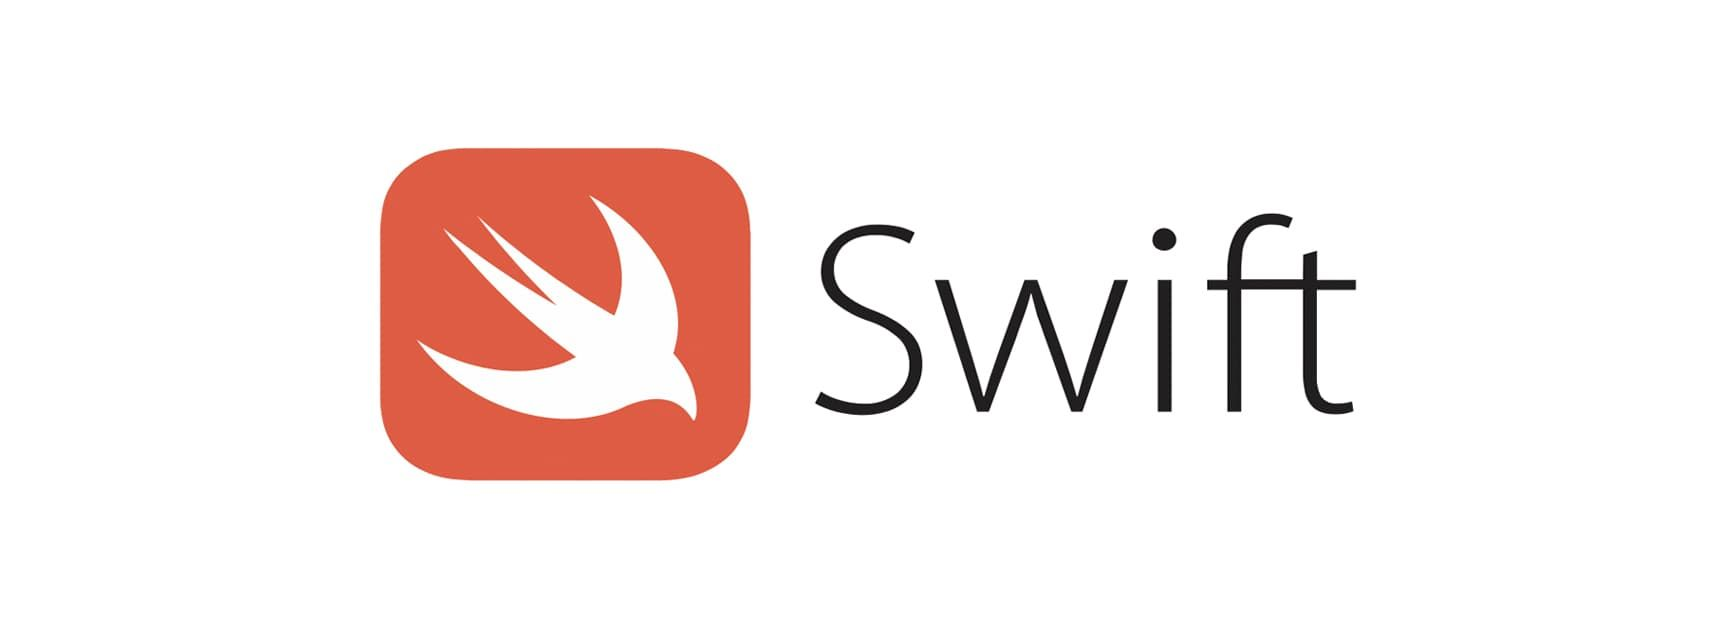
\includegraphics[width=0.4\textwidth]{swiftbird} 
    \caption{Het swift logo}
    \label{fig:swift}
\end{figure}
\subsubsection{Geschiedenis}
De ontwikkeling van swift is van start gegaan in 2010 door programmeur Chris Lattner. Swift voegde verschillende concepten samen uit andere programmeertalen zoals: Objective-C, Rust, Haskell, Python, C\#, CLU, en vele anderen. De eerste publieke Swift app is op 2 juni 2014 geschreven.

Een handleiding van 500 pagina's werd ook tijdens de WWDC beschikbaar gesteld in de iBooks Store en op de website van Apple.
\section{SwiftUI}
\autocite{AppleSwiftUI} SwiftUI is een door Apple ontwikkeld framework voor het bouwen van gebruikersinterfaces voor iOS, macOS, watchOS en tvOS, met behulp van de programmeertaal Swift. Het is ontworpen om de ontwikkeling van gebruikersinterfaces te vereenvoudigen door middel van een declaratieve syntax en een reeks krachtige tools en functies.
\begin{wrapfigure}{r}{0.3\textwidth}
    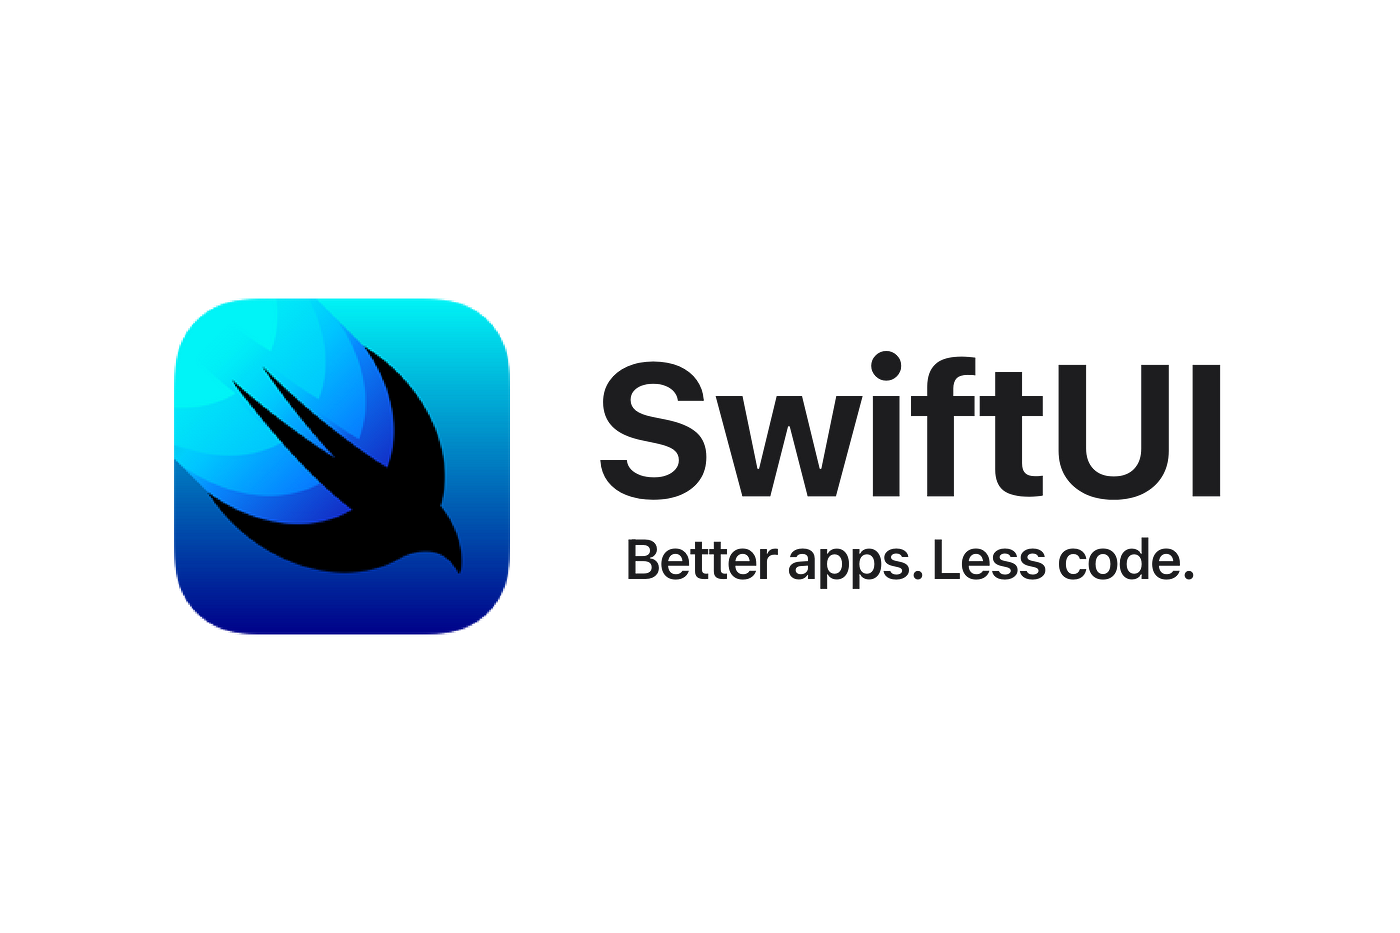
\includegraphics[width=0.3\textwidth]{swiftuibird} 
    \caption{Het swiftUI logo}
    \label{fig:swiftUI}
\end{wrapfigure}
Met SwiftUI kun je gebruikersinterfaces bouwen door middel van een reeks van herbruikbare en aanpasbare Views, waardoor je complexe UI-structuren kunt maken met minimale code. Het framework maakt gebruik van een state-driven architectuur, wat betekent dat de UI automatisch wordt bijgewerkt wanneer de toestand van de app verandert. In deze proef gaan we SwiftUI Views gebruiken om data aan mee te geven om zo performantie te tracken.

\subsection{Views}
\autocite{AppleSwiftViews} Views vormen de bouwstenen van elke SwiftUI-gebruikersinterface. Ze definiëren hoe content wordt weergegeven en gereageerd wordt op gebruikersinteracties. Views kunnen zowel elementaire interface-elementen (zoals tekst, knoppen en afbeeldingen) als complexere composities van deze elementen bevatten.

\begin{figure}[h]
    \begin{minipage}{0.5\textwidth}
        \begin{swift}[caption=Example of a view, label=view_example]
           struct MyView: View {
               var body: some View {
                   Text("Hello, World!")
               }
           }
        \end{swift}
    \end{minipage}%
    \hfill
    \begin{minipage}{0.45\textwidth}
        \centering
        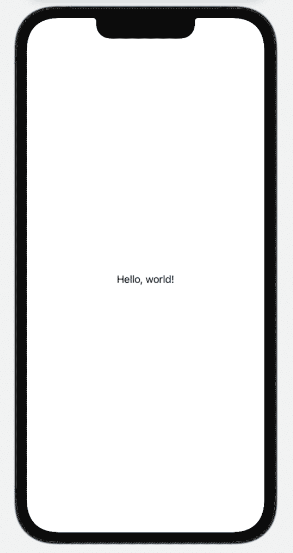
\includegraphics[height=130pt]{helloworldview}
        \caption{Example of a view}
        \label{fig:viewex1}
    \end{minipage}
\end{figure}

\section{Design Patterns}
Design patterns zijn oplossingen voor veelvoorkomende ontwerpproblemen in softwareontwikkeling. Ze bieden gestandaardiseerde en herbruikbare oplossingen voor problemen die zich vaak voordoen tijdens het ontwerpen van software. In Swift met SwiftUI zijn verschillende design patterns van toepassing om de ontwikkeling van robuuste en onderhoudbare apps te vergemakkelijken.

Design Patterns zijn belangerijk voor:
\begin{itemize}
    \item {\textbf{Herbruikbaarheid:} Design patterns bevorderen herbruikbaarheid van code.}
    \item {\textbf{Onderhoudbaarheid:} Ze maken de code gemakkelijker te begrijpen en te onderhouden.}
    \item {\textbf{Schaalbaarheid:} Door het gebruik van design patterns wordt het gemakkelijker om de app uit te breiden en nieuwe functies toe te voegen.}
    \item {\textbf{Testbaarheid:} Code die gebruikmaakt van design patterns is vaak gemakkelijker te testen vanwege de modulaire structuur.}
\end{itemize}
\autocite{MediumPatterns} Enkele belangerijke Design Patterns in Swift met SwiftUI zijn MVVM, MVC, MVP en VIPER.

\subsection{Model-View-ViewModel (MVVM)}
\autocite{MediumMVVM} MVVM is een design pattern dat veel wordt gebruikt in SwiftUI voor het scheiden van de logica van de gebruikersinterface van de onderliggende gegevens. Het bestaat uit drie hoofdcomponenten:
\begin{figure}[htbp]
    \centering
    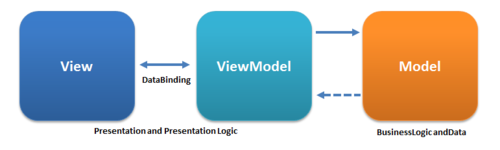
\includegraphics[width=1\textwidth]{MVVMPattern} 
    \caption{MVVM}
    \label{fig:mvvm}
\end{figure}
\begin{itemize}
    \item {\textbf{Model:} Het model bevat de gegevens van de app en de logica voor het manipuleren van die gegevens. Dit is waar de kernfunctionaliteit van de app zich bevindt.}
    \item {\textbf{View:} De view is verantwoordelijk voor het weergeven van de gebruikersinterface en het reageren op gebruikersinteracties. In SwiftUI worden views vaak passief gehouden en bevatten ze minimale logica.}
    \item {\textbf{ViewModel:} De viewmodel fungeert als een tussenliggende laag tussen het model en de view. Het voorziet de view van de gegevens die nodig zijn om te worden weergegeven en reageert op acties van de gebruiker. Het transformeert ook de gegevens van het model naar een vorm die gemakkelijk kan worden weergegeven in de view.}
\end{itemize}
De voordelen van MVVM zijn:
\begin{itemize}
    \item {\textbf{Scheiding van verantwoordelijkheden:} MVVM helpt bij het scheiden van de logica van de gebruikersinterface van de onderliggende gegevens, waardoor de code gemakkelijker te begrijpen en te onderhouden is. Dit zorgt ook voor een eenvoudigere uitbreidbaarheid en herbruikbaarheid van de code.}
    \item {\textbf{Testbaarheid:} Omdat de logica van de gebruikersinterface wordt gescheiden van de gegevenslogica, zijn de componenten gemakkelijker afzonderlijk te testen.}
\end{itemize}

\subsection{VIPER}
\autocite{MediumVIPER} VIPER is een design pattern dat staat voor View, Interactor, Presenter, Entity, en Router. Het is een architectureel patroon dat is ontworpen om de code van een app in verschillende lagen te verdelen om de onderhoudbaarheid en testbaarheid te verbeteren. Hier is een overzicht van de componenten:
\begin{figure}[htbp]
    \centering
    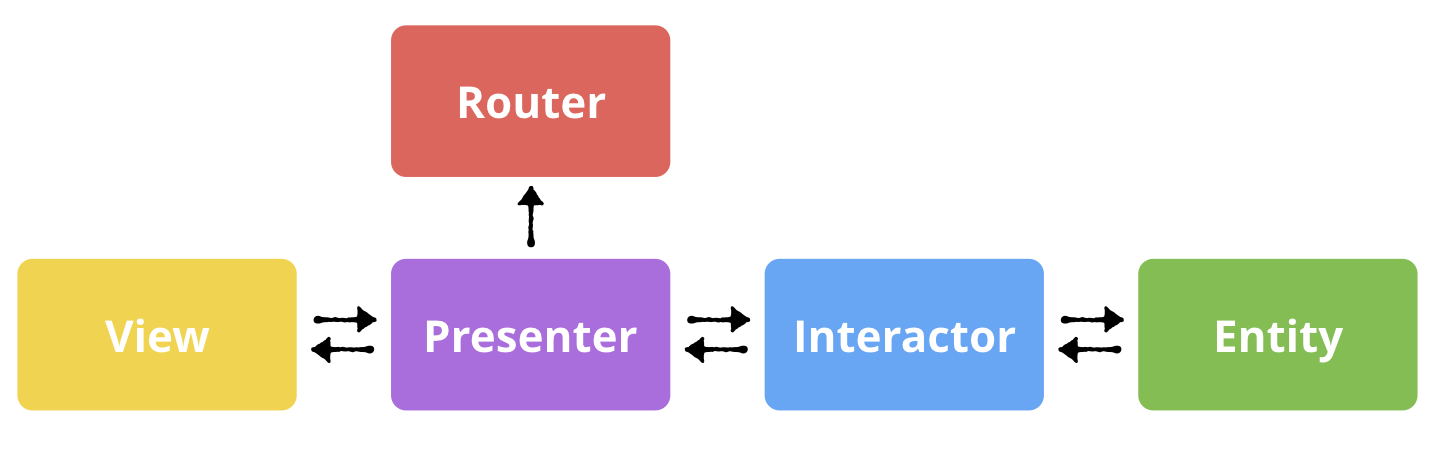
\includegraphics[width=1\textwidth]{viper} 
    \caption{viper}
    \label{fig:viper}
\end{figure}

\begin{itemize}
    \item {\textbf{View:} De view is verantwoordelijk voor het weergeven van de gebruikersinterface en het reageren op gebruikersinteracties, vergelijkbaar met MVVM.}
    \item {\textbf{Interactor:} De interactorcomponent bevat de businesslogica van de app. Het is verantwoordelijk voor het ophalen en verwerken van gegevens van externe bronnen, zoals een database of een netwerk.}
    \item {\textbf{Presenter:} De presenter fungeert als een tussenliggende laag tussen de interactor en de view. Het is verantwoordelijk voor het formatteren van de gegevens die zijn verkregen van de interactor en deze door te geven aan de view voor weergave.}
    \item {\textbf{Entity:} De entity bevat de gegevensmodellen van de app. Het vertegenwoordigt de entiteiten die worden gebruikt in de applicatie, zoals gebruikers, items, of andere objecten.}
    \item {\textbf{Router:} De router is verantwoordelijk voor het beheren van de navigatie binnen de app. Het bepaalt welke schermen moeten worden weergegeven en hoe deze moeten worden genavigeerd.}
\end{itemize}
Voordelen van VIPER zijn:
\begin{itemize}
    \item {\textbf{Schaalbaarheid:} Door de code in verschillende lagen te verdelen, maakt VIPER het gemakkelijker om de app uit te breiden en nieuwe functies toe te voegen.}
    \item {\textbf{Testbaarheid:} Elk onderdeel van VIPER kan afzonderlijk worden getest, waardoor het gemakkelijker wordt om bugs op te sporen en te repareren.}
\end{itemize}

\section{XCode Performance Trackers}

In deze proef gericht op het vergelijken van de performantie, rendering en lifescycles van views, zijn Xcode Profiler, Xcode Instruments en XCTest Metrics van onschatbare waarde. Xcode Profiler biedt een basisprofiel van views door CPU-, geheugen- en netwerkactiviteit te meten. Xcode Instruments gaat dieper met gedetailleerde analyses van CPU-, geheugen- en grafische prestaties, en kan rendercycli traceren. XCTest Metrics biedt automatische prestatiegegevensverzameling tijdens tests, wat helpt bij het identificeren van prestatieproblemen in views. Het integreren van bevindingen uit deze tools biedt een holistisch beeld van de view-prestaties, waardoor iteratieve optimalisatie mogelijk is voor een verbeterde gebruikerservaring en algehele app-prestaties.

\subsection{XCode Profiler}
Xcode Profiler is een krachtige tool die wordt geleverd als onderdeel van Apple's Xcode-ontwikkelomgeving. Het stelt ontwikkelaars in staat om de prestaties van hun iOS-, macOS-, watchOS- en tvOS-apps te meten en te optimaliseren. De profiler biedt inzicht in de runtime-gedrag van de app, inclusief CPU-gebruik, geheugenverbruik, netwerkactiviteit en meer. Met deze tool kunnen we in deze proef de performantie op basis van CPU-gebruik, geheugenverbruik, enz. gaan meten. 
\subsubsection{CPU-profiler}
Hiermee kan men het CPU-gebruik van een app analyseren. Men kan zien welke delen van de code veel CPU-tijd verbruiken en mogelijk optimalisaties doorvoeren om de prestaties te verbeteren.
\subsubsection{Geheugen-profiler}
Hiermee kan men het geheugenverbruik van een app analyseren. Men kan zien hoeveel geheugen de app gebruikt en hoe dit zich verhoudt tot verschillende delen van de code. Dit kan helpen bij het identificeren van geheugenlekken en het optimaliseren van de geheugenprestaties.
\subsubsection{Netwerkprofiler}
Hiermee kan men de netwerkactiviteit van de app analyseren. Men kan zien welke netwerkverzoeken de app maakt en hoe lang deze duren. Dit kan helpen bij het identificeren van trage netwerkverbindingen en het optimaliseren van de netwerkprestaties.
\subsubsection{Instruments}
Xcode Profiler maakt gebruik van Instruments, een krachtige tool voor het analyseren van de prestaties van een app. Instruments biedt verschillende instrumenten voor het meten van CPU-, geheugen- en netwerkprestaties, evenals voor het profileren van grafische en energiegebruik.


\subsection{Xcode Instruments}
Xcode Instruments is een krachtige tool die wordt geleverd als onderdeel van Apple's Xcode-ontwikkelomgeving. Het stelt ontwikkelaars in staat om diepgaande analyses uit te voeren van de prestaties en het gedrag van hun iOS-, macOS-, watchOS- en tvOS-apps. Met Instruments kunnen ontwikkelaars problemen met prestaties, geheugen, energieverbruik en meer opsporen en diagnosticeren. 

\subsubsection{Realtime monitoring}
Instruments biedt realtime monitoring van de prestaties van een app, waardoor men direct feedback krijgt over het gedrag van een app tijdens het gebruik. Dit stelt ontwikkelaars in staat om problemen snel op te sporen en te diagnosticeren terwijl ze optreden.
\subsubsection{Diepgaande analyse}
Met Instruments kunnen ontwikkelaars diepgaande analyses uitvoeren van de prestaties van hun app. Dit omvat gedetailleerde grafieken, tabellen en visuele hulpmiddelen om inzicht te krijgen in CPU-gebruik, geheugenverbruik, netwerkactiviteit, energieverbruik en meer.
\subsubsection{Tracing en Profiling}
Instruments ondersteunt zowel tracing als profiling van apps. Met tracing kan men het gedrag van een app volgen en analyseren gedurende een bepaalde periode, terwijl profiling men in staat stelt om specifieke aspecten van de prestaties van een app te meten en te optimaliseren.

\subsection{XCTest (Metrics)}
XCTest is een framework dat wordt gebruikt voor het schrijven en uitvoeren van tests in Swift- en Objective-C-gebaseerde applicaties voor iOS, macOS, watchOS en tvOS. Naast de standaard functionaliteit voor het schrijven van tests biedt XCTest ook XCTest Metrics, een functie die ontwikkelaars in staat stelt om verschillende prestatiegerelateerde metingen te verzamelen tijdens het uitvoeren van tests.

\subsubsection{Prestatiemetingen}
XCTest Metrics biedt verschillende metingen voor het evalueren van de prestaties van een app tijdens het uitvoeren van tests. Dit omvat metingen zoals CPU-gebruik, geheugenverbruik, netwerkactiviteit, energieverbruik en meer.
\subsubsection{Ingebouwde instrumenten}
XCTest Metrics maakt gebruik van de ingebouwde Instruments van Xcode om de prestaties van een app te meten. Dit stelt ontwikkelaars in staat om diepgaande analyses uit te voeren van de prestaties van hun app en om potentiële prestatieproblemen te identificeren.
\subsubsection{Grafische Weergave}
XCTest Metrics biedt een grafische weergave van de verzamelde prestatiegegevens, waardoor ontwikkelaars snel inzicht krijgen in de prestaties van hun app tijdens het uitvoeren van tests. Dit omvat grafieken, tabellen en andere visuele hulpmiddelen om trends en patronen te identificeren.
\subsubsection{Automatische Metingen}
XCTest Metrics voert automatisch metingen uit tijdens het uitvoeren van tests, waardoor ontwikkelaars zich kunnen concentreren op het schrijven van tests zonder zich zorgen te hoeven maken over het handmatig meten van prestaties. Dit maakt het gemakkelijker om consistente en betrouwbare metingen te verkrijgen.

\section{Annotations}
\subsection{@propertyWrapper}
\autocite{ApplePropertyWrapper} Een property wrapper voegt een scheidingslaag toe tussen de code die beheert hoe een property word opgeslagen en de code die een eigenschap definieert. Dit is interessant om te begrijpen omdat alle volgende annotaties property wrappers zijn.
\begin{swift}[caption=Example property wrapper code, label=property_wrapper_example]
    @propertyWrapper
    struct TwelveOrLess {
        private var number = 0
        var wrappedValue: Int {
            get { return number }
            set { number = min(newValue, 12) }
        }
    }
    
    struct SmallRectangle {
        @TwelveOrLess var height: Int
        @TwelveOrLess var width: Int
    }
    
    
    var rectangle = SmallRectangle()
    print(rectangle.height)
    // Prints "0"
    
    
    rectangle.height = 10
    print(rectangle.height)
    // Prints "10"
    
    
    rectangle.height = 24
    print(rectangle.height)
    // Prints "12"
\end{swift}


\subsection{@State}
\autocite{AppleState} State is een propertywrapper dat een waarde kan lezen en schrijven die word beheerd door SwiftUI. State word gebruikt voor de enige bron van de ``truth''(waarheid) voor een gegeven value type dat opgeslagen wordt binnen de view hierarchy.

\begin{swift}[caption=Example of @State code, label=state_example]
    struct PlayButton: View {
        @State private var isPlaying: Bool = false // Create the state.
        
        
        var body: some View {
            Button(isPlaying ? "Pause" : "Play") { // Read the state.
                isPlaying.toggle() // Write the state.
            }
        }
    }
\end{swift}


\subsection{@Binding}
\autocite{AppleBinding} Binding word gebruikt om een 2-way connection te leggen tussen een property dat data opslaat en een view dat data weergeeft. Een binding verbind een property met een bron van ``truth''(waarheid) in plaats van zelf de data op te slaan.

\begin{swift}[caption=Example of @Binding code, label=binding_example]
    struct PlayButton: View {
        @Binding var isPlaying: Bool
        
        
        var body: some View {
            Button(isPlaying ? "Pause" : "Play") {
                isPlaying.toggle()
            }
        }
    }
    
    struct PlayerView: View {
        var episode: Episode
        @State private var isPlaying: Bool = false
        
        
        var body: some View {
            VStack {
                Text(episode.title)
                .foregroundStyle(isPlaying ? .primary : .secondary)
                PlayButton(isPlaying: $isPlaying) // Pass a binding.
            }
        }
    }
\end{swift}


\subsection{@ObservableObject}
\autocite{AppleObservableObject} Een ObservableObject is een object dat veranderingen in zijn staat kan detecteren en hier melding(objectWillChange) van kan maken aan geïnteresseerde partijen, meestal via het Observer-patroon. Dit is een belangrijk concept in het kader van het ontwikkelen van applicaties met een reactieve programmeerstijl.

\subsubsection{Observer Pattern}
\autocite{MediumDesignPatterns} Dit patroon is een gedragspatroon waarbij een object, dat de 'observable' of 'subject' wordt genoemd, een lijst met afhankelijkheden bijhoudt, ook wel 'observers' genoemd. Wanneer het observable object verandert, worden alle geïnteresseerde observers op de hoogte gesteld van deze verandering.

\subsubsection{@Published}
\autocite{ApplePublished} De eenvoudigste manier om een object als observable te maken, is door de @Published-property wrapper te gebruiken voor eigenschappen die je wilt observeren. Wanneer de waarde van een eigenschap die is gemarkeerd met @Published verandert, zal het observable object automatisch melding maken van deze verandering aan alle geabonneerde observers.

\begin{swift}[caption=Example of implemented Observable Pattern, label=observable_example]
class Contact: ObservableObject {
    @Published var name: String
    @Published var age: Int
    
    
    init(name: String, age: Int) {
        self.name = name
        self.age = age
    }
    
    
    func haveBirthday() -> Int {
        age += 1
        return age
    }
}


let john = Contact(name: "John Appleseed", age: 24)
cancellable = john.objectWillChange
.sink { _ in
    print("(john.age) will change")
}
print(john.haveBirthday())
// Prints "24 will change"
// Prints "25"
\end{swift}

\subsection{@StateObject}
StateObject is een property wrapper in SwiftUI, waarmee je een instantie van een observable object kunt maken en behouden gedurende de levensduur van een specifieke SwiftUI View. Dit is handig wanneer je een observable object wilt gebruiken om de staat van een weergave te beheren, maar je wilt niet dat deze wordt gedeeld tussen verschillende instanties van dezelfde weergave.

\begin{swift}[caption=Example of StateObject, label=stateobject_example]
class MyData: ObservableObject {
    @Published var value: Int = 0
}

struct ContentView: View {
    @StateObject var data = MyData()
    
    var body: some View {
        VStack {
            ChildView(data: data)
            AnotherChildView(data: data)
        }
    }
}

struct ChildView: View {
    @ObservedObject var data: MyData
    
    var body: some View {
        VStack {
            Text("Value in ChildView: (data.value)")
            Button("Increment in ChildView") {
                data.value += 1
            }
        }
    }
}
struct AnotherChildView: View {
    @ObservedObject var data: MyData
    
    var body: some View {
        VStack {
            Text("Value in AnotherChildView: (data.value)")
            Button("Increment in AnotherChildView") {
                data.value += 1
            }
        }
    }
}

\end{swift}

\subsection{@Observable}
\autocite{AppleObservable} @Observable is een macro die gebruikt wordt in SwiftUI om het observer-patroon te implementeren. Dit patroon stelt een object in staat om een lijst van observers bij te houden en hen te notificeren over specifieke of algemene staatveranderingen. Deze macro is beschikbaar vanaf ios 17.0 en later. Deze macro is gemaakt om alle voorgaande macro's te vervangen.

\begin{swift}[caption=Example of Observable, label=Observable_example]
// ViewModel met @Observable macro
@Observable class SimpleViewModel {
    var text = "Hello World :)"
}

// SwiftUI View
struct SimpleView: View {
    @Environment(SimpleViewModel.self) var viewModel
    
    var body: some View {
        Text(viewModel.text)
    }
}
\end{swift}


\subsection{@Environment}
\autocite{AppleEnvironment} In SwiftUI biedt @Environment een mechanisme om waarden door te geven door de view-hiërarchie, zonder ze expliciet door te geven aan elke view als afzonderlijke eigenschappen. Het maakt gebruik van de omgeving van de View om gegevens te delen tussen Views in een hiërarchie. Dit is handig voor het doorgeven van gegevens die van toepassing zijn op de hele app of een deel ervan, zoals thema's, kleuren, taalinstellingen, enzovoort.


\begin{swift}[caption=Example of Observable, label=Observable_example]
struct ContentView: View {
    @Environment(\.colorScheme) var colorScheme
    
    var body: some View {
        VStack {
            Text("Current color scheme is (colorScheme)")
            ChildView()
        }
    }
}

struct ChildView: View {
    var body: some View {
        Text("This is a child view")
    }
}
\end{swift}

